%
% File acl2010.tex
%
% Contact  jshin@csie.ncnu.edu.tw or pkoehn@inf.ed.ac.uk
%%
%% Based on the style files for ACL-IJCNLP-2009, which were, in turn,
%% based on the style files for EACL-2009 and IJCNLP-2008...

%% Based on the style files for EACL 2006 by
%%e.agirre@ehu.es or Sergi.Balari@uab.es
%% and that of ACL 08 by Joakim Nivre and Noah Smith

\documentclass[11pt]{article}
\usepackage{cse595}
\usepackage{url}
\usepackage{latexsym}
\usepackage{graphicx}

%\setlength\titlebox{6.5cm}    % You can expand the title box if you
% really have to

\title{TagPandr: Tag exapansion for flickr images}

\author{Naresh Pratap Singh\\
  {\tt mail2naresh@gmail.com}  \And
  Rohith Menon\\
  {\tt rohithmenon@gmail.com} \And
  Sandesh Singh\\
  {\tt sandesh247@gmail.com}
  }

\date{}

\begin{document}
\maketitle
\begin{abstract}
We present an automatic method to suggest tags based on the existing tags provided by
users. We use co occurence statistics and wordnet to suggest tags in addition
to the existing tags, and use visual features to maintain the relevance of
the suggested tags to the image under consideration. We learn the visual features
for tags from Flickr image corpus. Experimental results show that better tags
  are suggested especially when the quality of original tags are low.
\end{abstract}

\section{Introduction}

A large number of photos are now available online, especially with photo sharing sites like
Flickr and Picassa. Annotation of images with relevant tags is a very useful feature especially
for image search, categorization and organization. While there has been advances in content
based analysis of images, scaling image data to web scale is a challenge.

In Flickr, tags are assigned by people who upload the photos. Tags irrelevant to the tasks of
image search and categorization happen to exist in the image tags. For eg: 2011 (the year) is generally
a tag associated with a photo taken on the new year of 2011. Similarly, model of camera is yet
another tag which is very specific to an image and not relevant to the content of it. Apart from
this, bulk upload of photo brings along with it the problem of bulk tagging. Especially for such
uploads, we find that a group of photos are tagged with the same set of tags. Such tagging, although
makes sense for the photo group as a whole, turns out to be irrelevant for many images in the group.
Poorly tagged images and under tagged images are other issues with commnunity tagging.

In this work, we present a method to automatically expand the given tags using text features and
rank the expanded tags with the visual features to highgly score those tags which are relevant to
the given image. We present multiple statistics about the suggested tags and also perform human
evaluation to compute the human perceived goodness of the suggested tags.

\section{Experimental Evaluation}
We performed experiments on flickr data set. Tags and images were separately downloaded using
flickr apis. We downloaded about 500,000 images from flickr belonging to categories: cat,
dog, train, aircraft, car, bus, places, crocodile, harley etc. We obtained 311,000 unique tags
corresponding to these images. Like mentioned before we filtered tags which contained numbers
and special characters. We found that such tags were not of much relevance to the images.

Evaluation of the tags would require some quantitative way of analysing quality. We evaluate
the tag quality automatically by two methods. Apart from these automatic methods, we also
perform human evaluation to score the tag quality.

\subsection{Original tag recall in top 5 suggested tags}
In this evaluation, we compute the number of tags in the original image tags that we suggest
in the top five tags automatically suggested by our method. The intuition behind this evaluation
is to make sure that the best tags we suggest have a good coverage of the original tags. Although
this method seems like a good measure of quality, the poor tags present in the original image
will cause this measure to degrade. Our method will fail to suggest original tags if there is
very less relevance with the given image. We calculate this measure of quality for tags generated
with text only features, visual only features and visual + text features. Table () tabulates the
experimental results.

Put the data.

From the table its clear that text features alone have better overlap with the given tags.
This is because, the original tags will also be suggested as part of the text co-occurrence
model. We see a decline in the scores with visual only attributes and text+visual attributes.
We attribute this to the fact that for visual features, the ranking of tags comes purely from
the gist or spatial pyramid features and hence the overlap with the original tags will be lesser.
For text+visual features, the ranking of tags push better tags to the top, which has lower overlap
with the original tags compared to text only features.

\subsection{Prediction of original tags removed from test images}
For this evaluation, we randomly remove 30 percent of the orignal tags from the test images. We
then pass these images through our pipeline and compute the number of tags suggested from the 
removed original tags in the top 20 of our suggested tags. The intuition behind this measure of
quality is to understand how well our models are able to simulate the quality of tags possessed
by original tags. This measure also has problems like mentioned before, but is a better measure
of quality because we look for the existence of the removed original tags in the suggested tag
set as a whole. We calculate this measure of quality for tags generated with text only features,
visual only features and visual + text only features. Table () tabulates the experimental results.

Put the data.

Put the inference.

\subsection{Evaluation of classifier One Vs Rest}
For this experimental setup, we trained a classifier one for each unique tag appearing atleast
10 times in a particular category. We experimented the one vs rest classifier with support vector
machines to learn the visual features for individual tags. It turns out that the performance of
this classifier is worse when compared with a single classifier with multi-class prediction.

\subsection{Human Evaluation}
The above mentioned statistics would provide a notion of quality of the tags suggested. But
we cannot compare it with the quality of the original tags. For this reason, we perform human
evaluation of the input tags for the given image. Human evaluation is peformed for each of the
output tag and the original tags. A score from 1 to 4 is assigned to each of the tag, 1 being
lowest on relevance scale and 4 being highest on relevance scale. During evaluation, tags which
were about places and not obvious in the image as part of content were scored as 1. For meta images,
(ie) images which are photos of the writings, visual features will be of very little use. But
text features would prove to be good. Human evaluation was performed for tags expanded with
text only features, visual only features and text+visual features. We also performed human 
evaluation of the original tags so that we could compare the scores of the original tags with
the suggested tags. Table() tabulates the results of the human evaluation.

Put the data.

We also found that when the number of tags in the image were less and those ones were very relevant,
the quality of tags expanded tended to be lesser. On the other hand when the original tags were bad,
we were able to suggest better quality tags. We studied the score pattern of original tags with respect
to the suggested tag. Figure() shows that when the original tag quality goes down, the suggested tag
quality goes up and vice versa.

Manuscripts must be in two-column format.  Exceptions to the
two-column format include the title, authors' names and complete
addresses, which must be centered at the top of the first page, and
any full-width figures or tables (see the guidelines in
Subsection~\ref{ssec:first}). {\bf Type single-spaced.}  Start all
pages directly under the top margin. See the guidelines later
regarding formatting the first page.  The manuscript should be
printed single-sided and its length
should not exceed the maximum page limit described in Section~\ref{sec:length}.

\subsection{Electronically-available resources}

ACL-2010 provides this description in \LaTeX2e (acl2010.tex) and PDF
format (acl2010.pdf), along with the \LaTeX2e style file used to
format it (acl2010.sty) and an ACL bibliography style
(acl.bst). These files are all available at
\url{http://nlp.csie.ncnu.edu.tw/~shin/acl2010/publication/doc/stylefiles/}. A Microsoft Word
template file (acl2010.dot) is also available at the same URL. We
strongly recommend the use of these style files, which have been
appropriately tailored for the ACL-2010 proceedings. If you have an
option, we recommend that you use the \LaTeX2e version. \textbf{If you will be
using the Microsoft Word template, we suggest that you anonymize your
source file so that the pdf produced does not retain your identity.}
This can be done by removing any personal information from your source
document properties.



\subsection{Format of Electronic Manuscript}
\label{sect:pdf}

For the production of the electronic manuscript you must use Adobe's
Portable Document Format (PDF). This format can be generated from
postscript files. On Linux/Unix systems, you can use {\tt ps2pdf} for
this purpose. In Microsoft Windows, you can use Adobe's Distiller
or GSview (File$<$Convert$<$pdfwrite); if you have \textit{cygwin}
installed, you can use \textit{dvipdf} or \textit{ps2pdf}. Note that
some word processing programs generate PDF which may not include all
the necessary fonts (esp. tree diagrams, symbols). When you print or
create the PDF file, there is usually an option in your printer setup
to include none, all or just non-standard fonts.  Please make sure
that you select the option of including ALL the fonts. {\em Before
sending it, test your PDF by printing it from a computer different
from the one where it was created.} Moreover, some word processors may
generate very large postscript/PDF files, where each page is rendered
as an image. Such images may reproduce poorly. In this case, try
alternative ways to obtain the postscript and/or PDF. One way on some
systems is to install a driver for a postscript printer, send your
document to the printer specifying ``Output to a file'', then convert
the file to PDF.

It is of utmost importance to specify the A4 format (21 cm
x 29.7 cm) when formatting the paper. When working with
{\tt dvips}, for instance, one should specify {\tt -t a4}.

Print-outs of the PDF file on A4 paper should be identical to the
hardcopy version. If you cannot meet the above requirements about the
production of your electronic submission, please contact the
publication chairs above as soon as possible.


\subsection{Layout}
\label{ssec:layout}

Format manuscripts two columns to a page, in the manner these
instructions are formatted. The exact dimensions for a page on A4
paper are:

\begin{itemize}
\item Left and right margins: 2.5 cm
\item Top margin: 2.5 cm
\item Bottom margin: 2.5 cm
\item Column width: 7.7 cm
\item Column height: 24.7
\item Gap between columns: 0.6 cm
\end{itemize}

Papers should not be formatted for any other paper size.
% Removed by KO  we are not accepting printed papers any more!!!
%  Exceptionally,
% authors for whom it is \emph{impossible} to print on A4 paper may use
% \emph{US Letter} paper. In this case, they should keep the \emph{top}
% and \emph{left} margins as given above, use the same column width,
% height and gap, and modify the bottom and right margins as
% necessary. Note that the text will no longer be centered.

\subsection{Fonts}

For reasons of uniformity, Adobe's {\bf Times Roman} font should be
used. In \LaTeX2e{} this is accomplished by putting

\begin{quote}
\begin{verbatim}
\usepackage{times}
\usepackage{latexsym}
\end{verbatim}
\end{quote}
in the preamble. If Times Roman is unavailable, use {\bf Computer
  Modern Roman} (\LaTeX2e{}'s default).  Note that the latter is about
  10\% less dense than Adobe's Times Roman font.


\begin{table}[h]
\begin{center}
\begin{tabular}{|l|rl|}
\hline \bf Type of Text & \bf Font Size & \bf Style \\ \hline
paper title & 15 pt & bold \\
author names & 12 pt & bold \\
author affiliation & 12 pt & \\
the word ``Abstract'' & 12 pt & bold \\
section titles & 12 pt & bold \\
document text & 11 pt  &\\
captions & 11 pt & \\
abstract text & 10 pt & \\
bibliography & 10 pt & \\
footnotes & 9 pt & \\
\hline
\end{tabular}
\end{center}
\caption{\label{font-table} Font guide. }
\end{table}

\subsection{The First Page}
\label{ssec:first}

Center the title, author's name(s) and affiliation(s) across both
columns. Do not use footnotes for affiliations. Do not include the
paper ID number assigned during the submission process. Use the
two-column format only when you begin the abstract.

{\bf Title}: Place the title centered at the top of the first page, in
a 15-point bold font. (For a complete guide to font sizes and styles, see Table~\ref{font-table}.) Long titles should be typed on two lines without
a blank line intervening. Approximately, put the title at 2.5 cm from
the top of the page, followed by a blank line, then the author's
names(s), and the affiliation on the following line. Do not use only
initials for given names (middle initials are allowed). Do not format surnames
in all capitals (e.g., use ``Schlangen'' not ``SCHLANGEN'').
Do not format title and section headings in all capitals as well
except for proper names (such as ``BLEU'') that are conventionally
in all capitals.
The affiliation should contain the author's complete address, and if
possible, an electronic mail address. Leave about 2 cm between the
affiliation and the body of the first page.
The title, author names and addresses should be completely
identical to those entered to the electronical paper submission
website in order to maintain the consistency of author information
among all publications of the conference.

{\bf Abstract}: Type the abstract at the beginning of the first
column. The width of the abstract text should be smaller than the
width of the columns for the text in the body of the paper by about
0.6 cm on each side. Center the word {\bf Abstract} in a 12 point bold
font above the body of the abstract. The abstract should be a concise
summary of the general thesis and conclusions of the paper. It should
be no longer than 200 words.

{\bf Text}: Begin typing the main body of the text immediately after
the abstract, observing the two-column format as shown in
the present document.

{\bf Indent} when starting a new paragraph. Use 11 points for text and
subsection headings, 12 points for section headings and 15 points for
the title.

\subsection{Sections}

{\bf Headings}: Type and label section and subsection headings in the
style shown on the present document.  Use numbered sections (Arabic
numerals) in order to facilitate cross references. Number subsections
with the section number and the subsection number separated by a dot,
in Arabic numerals.

{\bf Citations}: Citations within the text appear
in parentheses as~\cite{Gusfield:97} or, if the author's name appears in
the text itself, as Gusfield~\shortcite{Gusfield:97}.
Append lowercase letters to the year in cases of ambiguity.
Treat double authors by using both authors' last names (e.g.,
\cite{Aho:72}, but use \emph{et al.} when more than two authors are
involved.  (e.g. \cite{Chandra:81})
Collapse multiple citations (e.g., \cite{Gusfield:97,Aho:72}.) Also
refrain from using full citations as sentence constituents. We suggest
that instead of
\begin{quote}
  ``\cite{Gusfield:97} showed that ...''
\end{quote}
you use
\begin{quote}
``Gusfield \shortcite{Gusfield:97}   showed that ...''
\end{quote}

If you are using the provided \LaTeX{} and Bib\TeX{} style files, you
can use the command \verb|\newcite| to get ``author (year)'' citations.

As reviewing will be double-blind, the submitted version of the papers should not include the
authors' names and affiliations. Furthermore, self-references that
reveal the author's identity, e.g.,
\begin{quote}
``We previously showed \cite{Gusfield:97} ...''
\end{quote}
should be avoided. Instead, use citations such as
\begin{quote}
``Gusfield \shortcite{Gusfield:97}
previously showed ... ''
\end{quote}

Please do not  use anonymous
citations and  do not include acknowledgements when submitting your papers. Papers that do not conform
to these requirements may be rejected without review.

\textbf{References}: Gather the full set of references together under
the heading {\bf References}; place the section before any Appendices,
unless they contain references. Arrange the references alphabetically
by first author, rather than by order of occurrence in the text.
Provide as complete a citation as possible, using a consistent format,
such as the one for {\em Computational Linguistics\/} or the one in the
{\em Publication Manual of the American
Psychological Association\/}~\cite{APA:83}.  Use of full names for
authors rather than initials is preferred.  A list of abbreviations
for common computer science journals can be found in the ACM
{\em Computing Reviews\/}~\cite{ACM:83}.

The \LaTeX{} and Bib\TeX{} style files provided roughly fit the
American Psychological Association format, allowing regular citations,
short citations and multiple citations as described above.

{\bf Appendices}: Appendices, if any, directly follow the text and the
references (but see above).  Letter them in sequence and provide an
informative title: {\bf Appendix A. Title of Appendix}.

\textbf{Acknowledgement} section should go as a last section immediately
before the references.  Do not number the acknowledgement section.

\subsection{Footnotes}

{\bf Footnotes}: Put footnotes at the bottom of the page and use 9
points text. They may be numbered or referred to by asterisks or other
symbols.\footnote{This is how a footnote should appear.} Footnotes
should be separated from the text by a line.\footnote{Note the line
separating the footnotes from the text.}

\subsection{Graphics}

{\bf Illustrations}: Place figures, tables, and photographs in the
paper near where they are first discussed, rather than at the end, if
possible.  Wide illustrations may run across both columns.  Color
illustrations are discouraged, unless you have verified that
they will be understandable when printed in black ink.

{\bf Captions}: Provide a caption for every illustration; number each one
sequentially in the form:  ``Figure 1. Caption of the Figure.'' ``Table 1.
Caption of the Table.''  Type the captions of the figures and
tables below the body, using 11 point text.

\section{Translation of non-English Terms}

It is also advised to supplement non-English characters and terms
with appropriate transliterations and/or translations
since not all readers understand all such characters and terms.
Inline transliteration or translation can be represented in
the order of: original-form transliteration ``translation''.

\section{Implementation}
\begin{figure*}
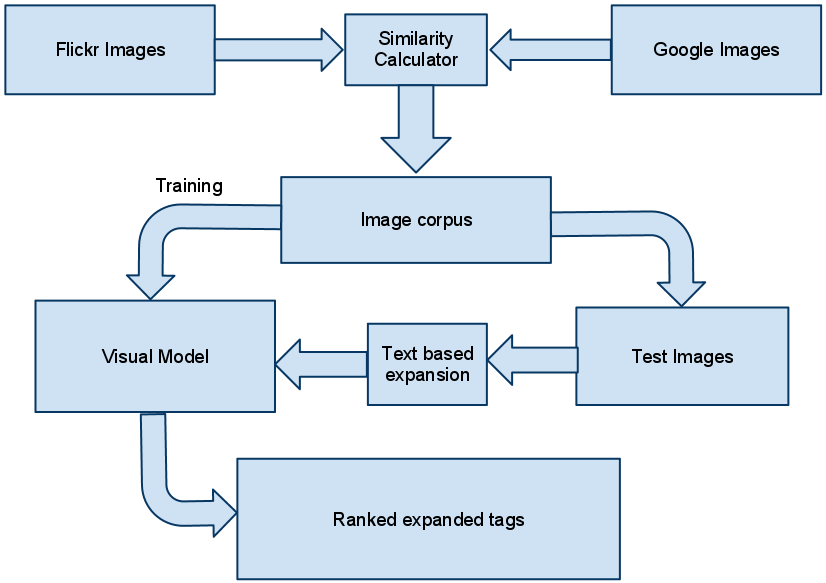
\includegraphics[width=0.8\textwidth]{model.png}
\end{figure*}

We downloaded [a lot of] Flickr images, pertaining to pre-selected categories.
For each category, we performed a Google search to get canonical images for
those vcategories. We found that for any given keyword, the results returned
by Google were consistently more represnetative of that category. We used the
most similar Flickr images (based on Euclidean distance of the gist vectors)
for training.

\begin{figure*}
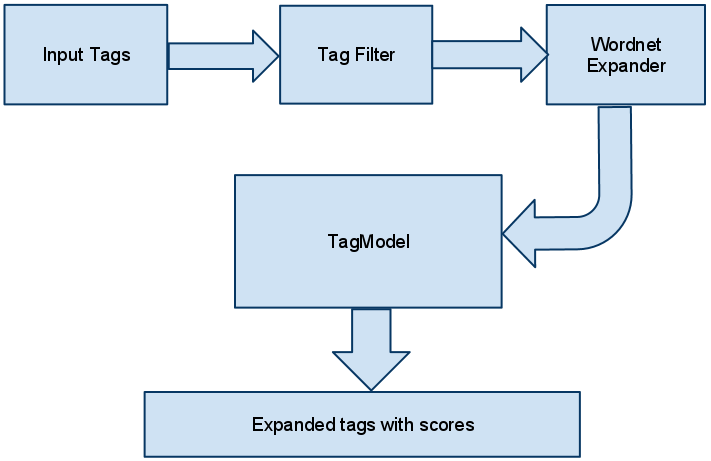
\includegraphics[width=0.8\textwidth]{tagExpansion.png}
\end{figure*}

We trained two models, a tag model and a visual model trained on the visual
features of the images. We used two visual features, gist vectors and spatial
pyramid based on [someones] method. We build a bayes model for the tags using
the co-occurence statistics from the tags of the training images. We evaluated
multiple calssifiers on the visual features, including smo and bayesian net.


\section*{Acknowledgments}

Do not number the acknowledgment section. Do not include this section
when submitting your paper for review.
%\bibliographystyle{acl}
% you bib file should really go here
%\bibliography{ref}

\begin{thebibliography}{}

\bibitem[\protect\citename{Aho and Ullman}1972]{Aho:72}
Alfred~V. Aho and Jeffrey~D. Ullman.
\newblock 1972.
\newblock {\em The Theory of Parsing, Translation and Compiling}, volume~1.
\newblock Prentice-{Hall}, Englewood Cliffs, NJ.

\bibitem[\protect\citename{{American Psychological Association}}1983]{APA:83}
{American Psychological Association}.
\newblock 1983.
\newblock {\em Publications Manual}.
\newblock American Psychological Association, Washington, DC.

\bibitem[\protect\citename{{Association for Computing Machinery}}1983]{ACM:83}
{Association for Computing Machinery}.
\newblock 1983.
\newblock {\em Computing Reviews}, 24(11):503--512.

\bibitem[\protect\citename{Chandra \bgroup et al.\egroup }1981]{Chandra:81}
Ashok~K. Chandra, Dexter~C. Kozen, and Larry~J. Stockmeyer.
\newblock 1981.
\newblock Alternation.
\newblock {\em Journal of the Association for Computing Machinery},
  28(1):114--133.

\bibitem[\protect\citename{Gusfield}1997]{Gusfield:97}
Dan Gusfield.
\newblock 1997.
\newblock {\em Algorithms on Strings, Trees and Sequences}.
\newblock Cambridge University Press, Cambridge, UK.

\end{thebibliography}

\end{document}
